\appendix
\section{appendix}
\label{sec:appendix}
\begin{figure}[htp]
    \centering
    \includegraphics[width=0.6\textwidth]{figures/UWRT Team Structure.png}
    \caption{
        UWRT employs a three-level organizational structure. The Team Lead oversees primary communication with university administrators and sponsors, while the Safety Captain ensures compliance with safety standards. The Business Lead manages outreach initiatives and sponsorship agreements. Senior members form an Architecture Decision Committee that reviews and approves all architectural decisions and purchase requests. The third level consists of general team members across mechanical, electrical, firmware, software, and business disciplines who continuously develop and implement new rover features using state-of-the-art algorithms.
    }
    \label{fig:uwrt_team_structure}
\end{figure}

\begin{figure}[htp]
    \centering
    \includegraphics[width=0.8\textwidth]{figures/UWRT PDR Balance Sheet.png}
    \caption{
        UWRT Season 2026 Budget: income (left) and expenses by project (right).
    }
    \label{fig:uwrt_balance}
\end{figure}

% add Mechanical; add testing and integration with detail; add electrical tasks.
% add better caption
\begin{figure}[htp]
    \centering
    \includegraphics[width=0.8\textwidth]{figures/S26 UWRT Gantt Chart.png}
    \caption{
        The Gantt chart illustrates the UWRT S26 project timeline and is organized into two sections. The top section displays key project deadlines, color-coded as follows: red indicates URC competition deadlines, orange marks system functionality milestones, and yellow represents project completion deadlines. The bottom section presents the detailed task timeline for each subteam—Mechanical, Electrical, Firmware, Software, Integration, Testing, and specialized subsystems (Drivetrain, Arm, Science, and Communications)—with color-coded task tracking. The team has structured the project around three major milestones. First, the team focuses on validating the functionality of all primary components, including both commercial off-the-shelf and custom-designed parts. Following PDR document submission, the team will lock in the system architecture for the season. The second milestone targets the system's minimal viable product (MVP). Finally, the team will conduct fine-tuning and stress testing to optimize system performance for the University Rover Challenge competition.
    }
    \label{fig:uwrt_gantt}
\end{figure}

% Where is the Science Module and Ground Station
\begin{figure}[htp]
    \centering
    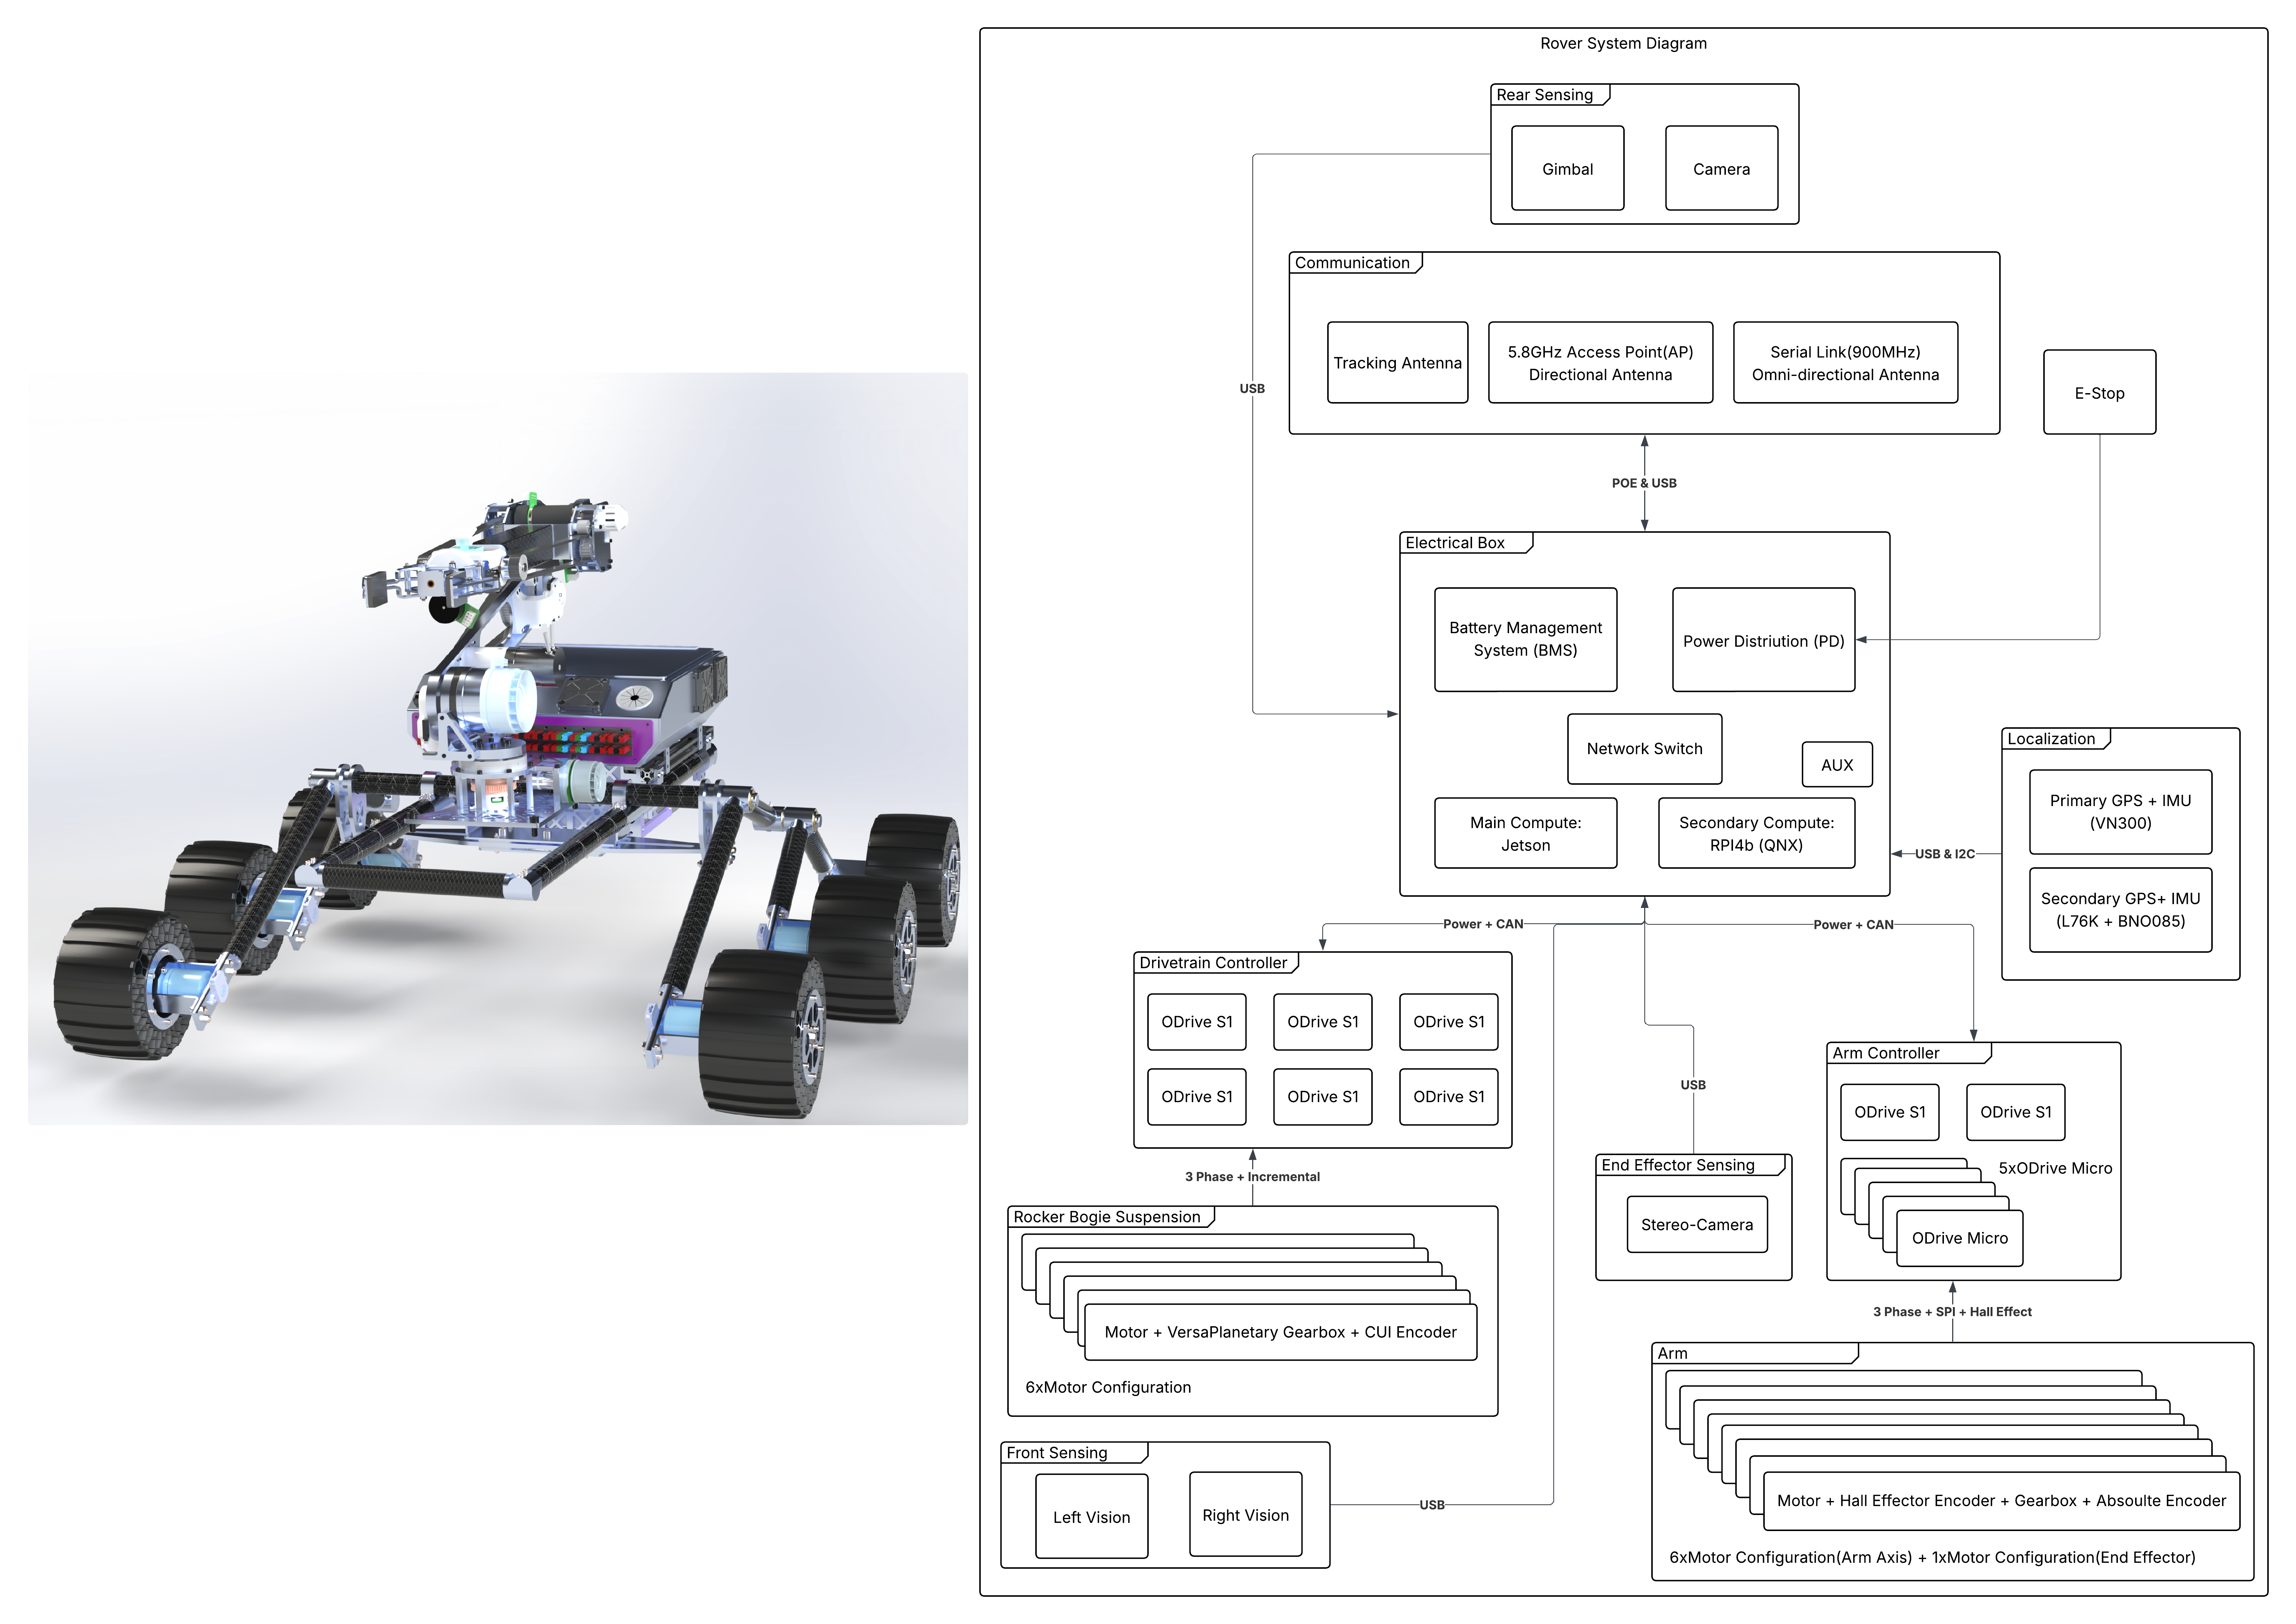
\includegraphics[width=0.8\textwidth]{figures/Rover System Diagram.png}
    \caption{
        This figure shows the main system diagram for the whole rover system. 
        The center is the Electrical Box containing all the main electronics. 
        BMS is for cell balancing. 
        PD is for over-voltage protection, over-current protection, and state of charge monitoring. 
        Jetson is our main controller solving all the kinematics. 
        Raspberry Pi 4B loaded with QNX serves as an IO expansion board and low-level controller. 
        Communication Module transmits UDP packets and communicates with the ground station. 
        The Rear Sensing Module serves as an overview camera for livestreaming the rover status to the ground station. 
        E-Stop performs the critical safety functionality and cuts the high power rail under emergency. 
        Localization has a dual GPS + IMU configuration providing high accuracy location results after sensor fusion. 
        Front Sensing uses two cameras to perform obstacle avoidance and path planning. 
        Drivetrain and Arm systems are described in their own architecture diagrams.
    }
    \label{fig:rover_sys_arch}
\end{figure}